\section{Que doit offrir un ERP~?}

Le terme ERP vient de l’anglais <<~Enterprise Ressource Planning~>> et il a été traduit en français par l’acronyme PGI~:~Progiciel de Gestion Intégré.
Il se définit comme un groupe de modules relié à une base de données unique.
C'est un outil utilisé par la totalité des employés d'une entreprise.
Il permet de faciliter les flux d'informations et de coordonner toutes les ressources et activités de la compagnie.
Les fonctions qui sont typiquement supportées par un tel outil incluent la fabrication, l'inventaire, les expéditions, la logistique, la distribution, la facturation, la comptabilité, la gestion des clients et des ressources humaines.
Il offre un environnement de travail uniforme et consistant pour tous les employés.

\FloatBarrier
\begin{figure}[h!]
    \begin{center}
        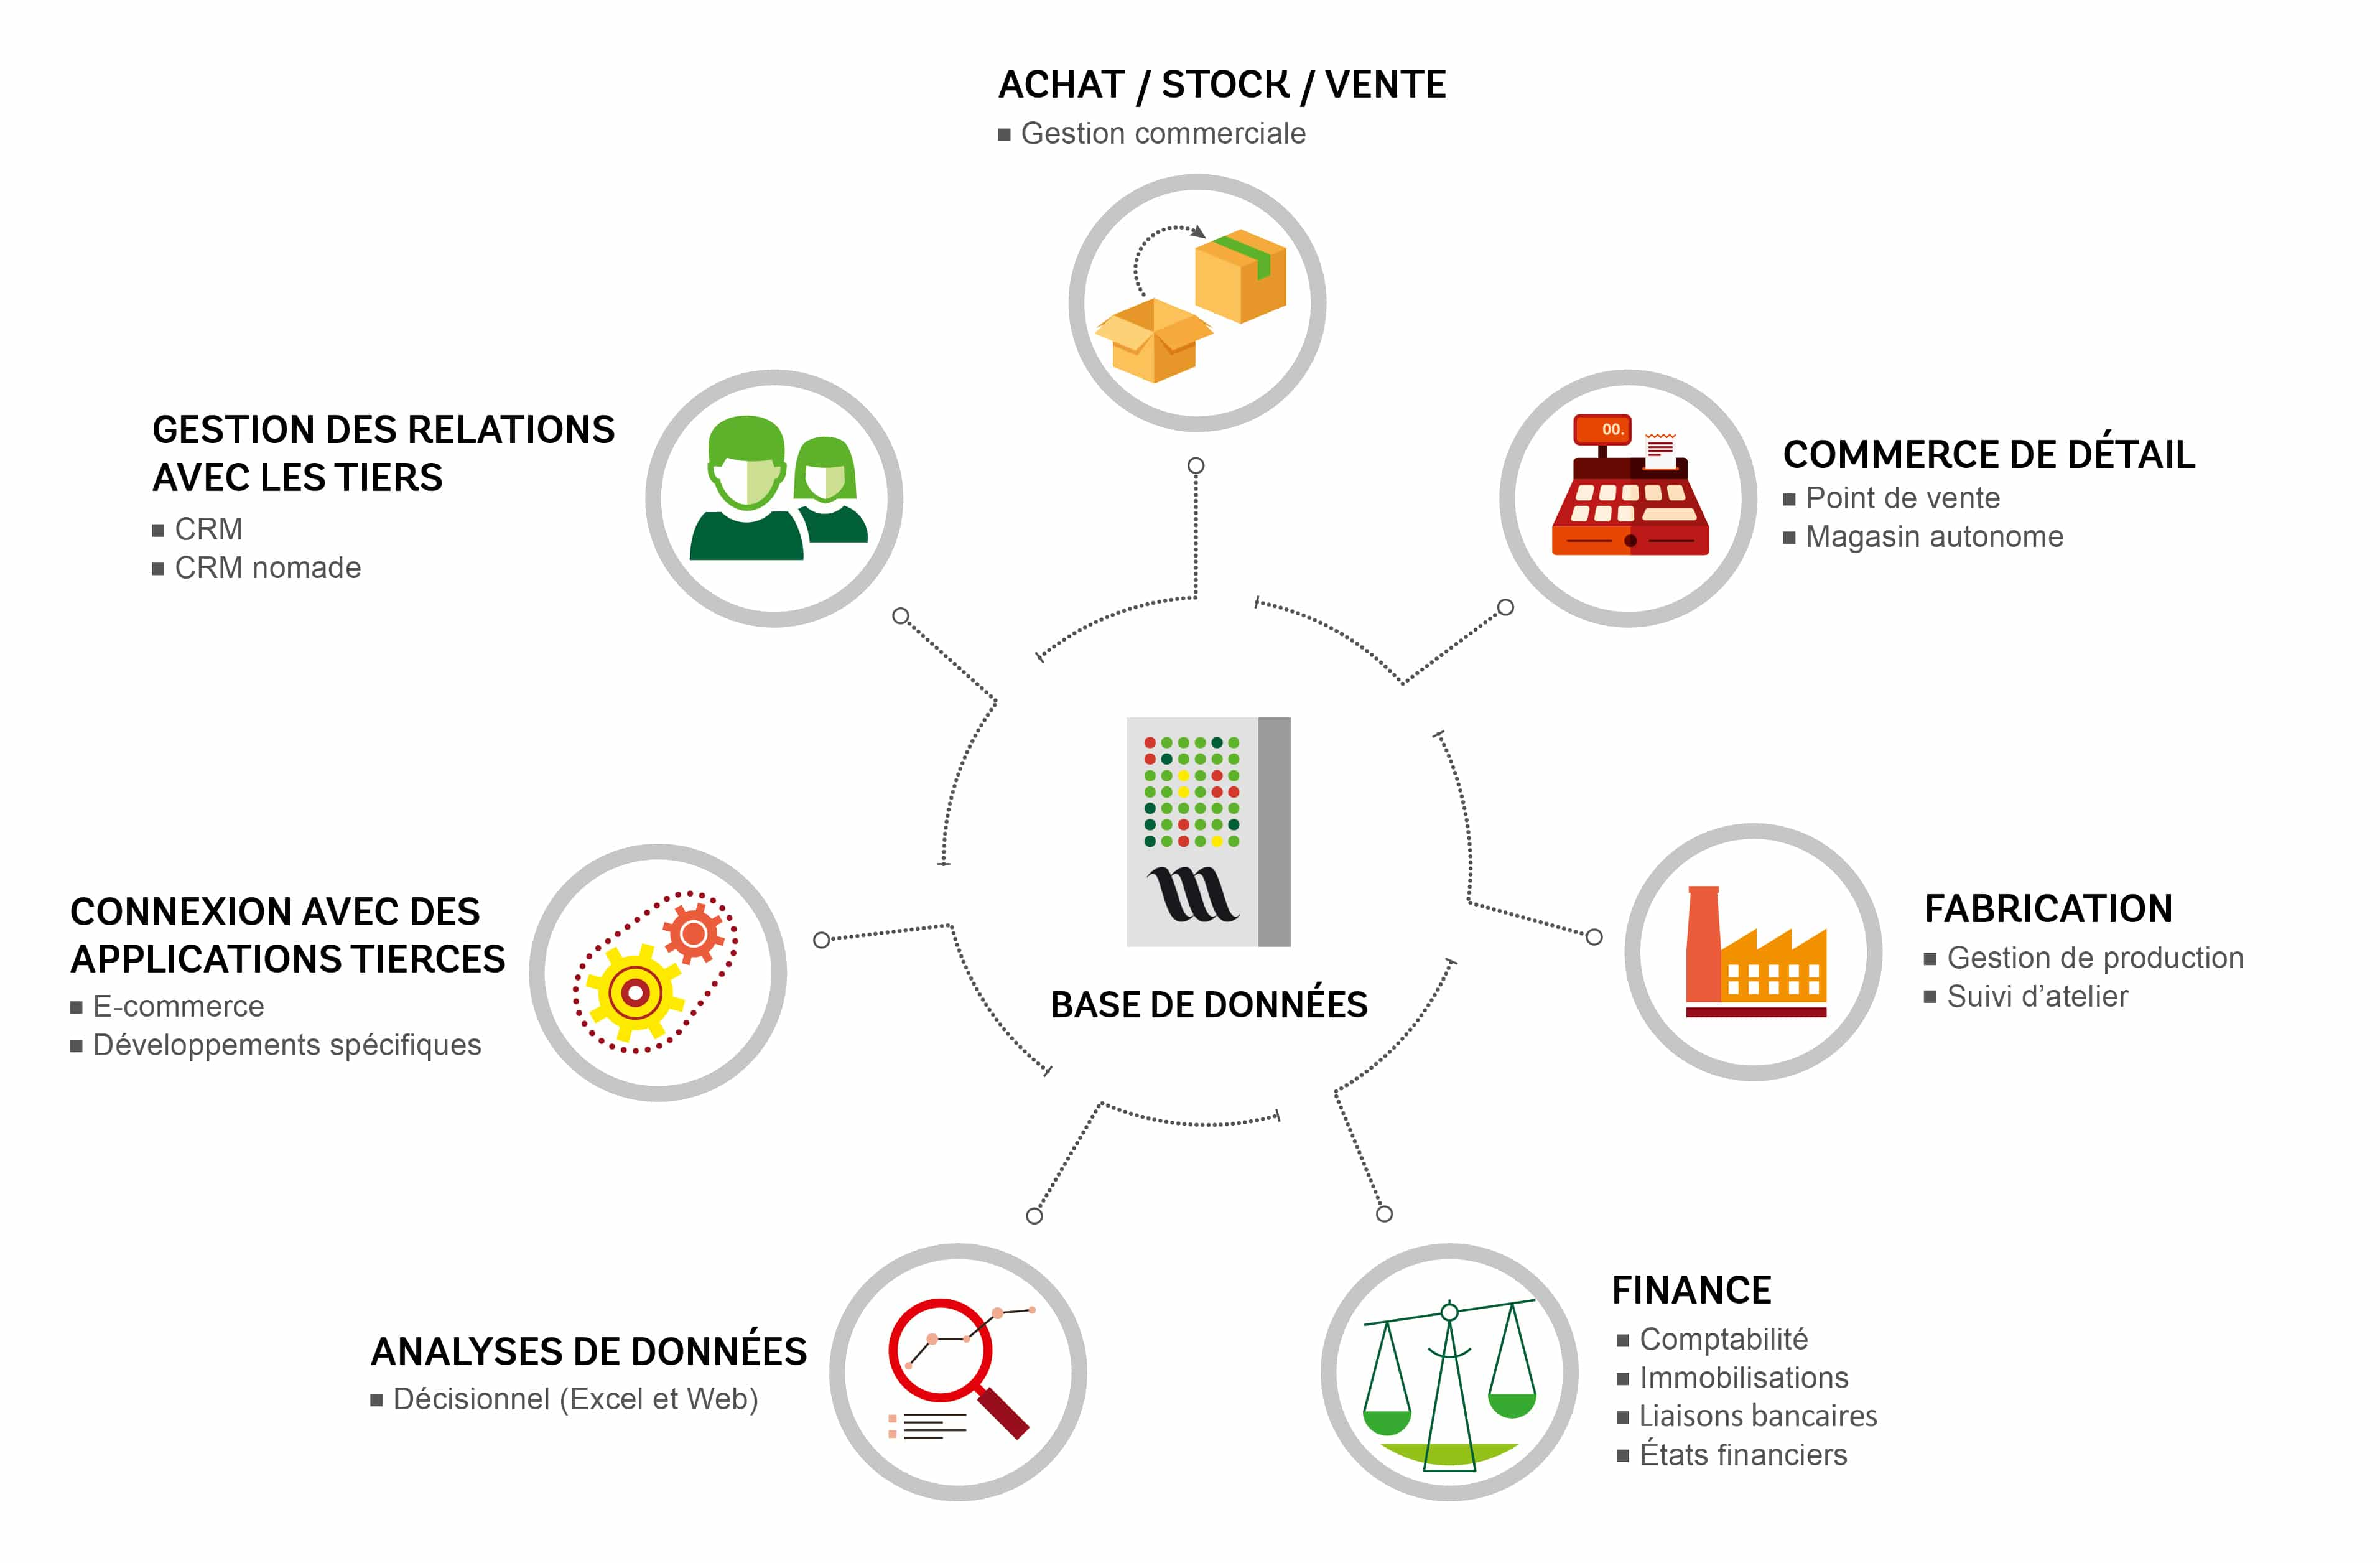
\includegraphics[width = 0.7\textwidth]{offre_wavesoft}
    \end{center}
    \caption{Les services couverts par la plupart des ERP}
    \label{figure:erp}
\end{figure}
\FloatBarrier

De toutes les technologies pouvant être déployées au sein d'une compagnie, à l'heure actuelle c'est un ERP qui a le plus de potentiel et l'impact le plus direct sur la réduction des coûts dans la compagnie.
Une étude de 2010, menée par le groupe \textsc{Aberdeen} \cite{erp_sme}, sur de petites et moyennes entreprises a permis de mettre en avant les facteurs les plus importants pour l'utilisation d'un ERP au sein de celles-ci.
La distribution de ces facteurs est affichée ci-dessous. 

\FloatBarrier
\begin{figure}[h!]
    \begin{center}
        \begin{bchart}[steps={10,20,30,40,50},max=50]
            \bcbar[label=Réduire les coûts, color=col_sections]{45}
            \bcskip{5pt}
            \bcbar[label=Simplifier le travail, color=col_sections]{36}
            \bcskip{5pt}
            \bcbar[label=Gérer les attentes de croissance, color=col_sections]{28}
            \bcskip{5pt}
            \bcbar[label=Améliorer les temps de réponse des clients, color=col_sections]{27}
            \bcskip{5pt}
            \bcbar[label=Régler les problèmes d'interopérabilité entre sites, color=col_sections]{19}
            \bcskip{5pt}
            \bcbar[label=Faciliter l'innovation, color=col_sections]{18} \bcskip{5pt}
            \bcxlabel{Pourcentage (\%)}
        \end{bchart}
    \end{center}
    \caption{Distribution des principaux facteurs d'adoption d'un ERP dans une PME}
    \label{figure:erp_bar}
\end{figure}
\FloatBarrier

Au sein de \textsc{Disa} avant l'année 2000, l'entreprise avait besoin d'un système permettant de mieux suivre ses données (clients, devis, commandes, factures) et également un suivi de la fabrication, jusqu'alors inexistant.
La compagnie décida donc de faire l'acquisition de l'ERP ASAP, produit par la société \textsc{Innetis}.
Sa mise en place dura deux ans et l'outil devint rapidement indispensable au bon fonctionnement de \textsc{Disa}.
Suite au vieillissement d'ASAP, le développement de plus en plus d'applications sous \textsc{Disanet} entraîna la perte des avantages de l'utilisation d'un ERP et c'est pour cette raison que le service informatique commença le développement de \textsc{Sigma}.
